\documentclass[12pt]{article} 

\usepackage{fullpage}
\usepackage{bookmark}
\usepackage{amsmath}
\usepackage{amssymb}
\usepackage[dvipsnames]{xcolor}
\usepackage{hyperref} % for the URL
\usepackage[shortlabels]{enumitem}
\usepackage{mathtools}
\usepackage[most]{tcolorbox}
\usepackage[amsmath,standard,thmmarks]{ntheorem} 
\usepackage{physics}
\usepackage{pst-tree} % for the trees
\usepackage{verbatim} % for comments, for version control
\usepackage{tabu}
\usepackage{tikz}
\usepackage{float}
\usepackage{siunitx}
\usepackage{physunits}
\usepackage{pgfplots}

% From the Plot video

\usepackage[LGR,T1]{fontenc}
\usepackage[utf8]{inputenc}
\usepackage{lmodern}
\usepackage{microtype}
\usepackage{upgreek}
\usepackage[misc]{ifsym}

\usepackage{pgfplots}
	\usetikzlibrary{
		calc,
		patterns,
		positioning
	}
	\pgfplotsset{
		compat=1.16,
		samples=200,
		clip=false,
		my axis style/.style={
			axis x line=middle,
			axis y line=middle,
			legend pos=outer north east,
			axis line style={
				->,
			},
			legend style={
				font=\footnotesize
			},
			label style={
				font=\footnotesize
			},
			tick label style={
				font=\footnotesize
			},
			xlabel style={
				at={
					(ticklabel* cs:1)
				},
				anchor=west,
				font=\footnotesize,
			},
			ylabel style={
				at={
					(ticklabel* cs:1)
				},
				anchor=west,
				font=\footnotesize,
			},
			xlabel=$t$,
			ylabel=$\vec v (\m \tx{[East]})$
		},
	}
	\tikzset{
		>=stealth
	}


    \pgfplotsset{my style/.append style={axis x line=middle, axis y line=
           middle, xlabel={$t$}, axis equal }}

%%% Tables and figures packages

\usepackage{float}
\usepackage{caption}
	\captionsetup{
		format=plain,
		labelfont=bf,
		font=small,
		justification=centering
	}
	
%%% Numbers and sets

\newcommand{\E}{\mathrm{e}}
\newcommand{\tx}[1]{\text{#1}}


% floor, ceiling, set
\DeclarePairedDelimiter{\ceil}{\lceil}{\rceil}
\DeclarePairedDelimiter{\floor}{\lfloor}{\rfloor}
\DeclarePairedDelimiter{\set}{\lbrace}{\rbrace}
\DeclarePairedDelimiter{\iprod}{\langle}{\rangle}

\DeclareMathOperator{\Int}{int}
\DeclareMathOperator{\mean}{mean}

% commonly used sets
\newcommand{\R}{\mathbb{R}}
\newcommand{\Nat}{\mathbb{N}}
\newcommand{\Q}{\mathbb{Q}}
\renewcommand{\P}{\mathbb{P}}

\newcommand{\sset}{\subseteq}


\theoremstyle{break}
\theorembodyfont{\upshape}

\newtheorem{thm}{Theorem}[subsection]
\tcolorboxenvironment{thm}{
enhanced jigsaw,
colframe=Dandelion,
colback=White!90!Dandelion,
drop fuzzy shadow east,
rightrule=2mm,
sharp corners,
before skip=10pt,after skip=10pt
}

\newtheorem{cor}{Corollary}[thm]
\tcolorboxenvironment{cor}{
boxrule=0pt,
boxsep=0pt,
colback={White!90!RoyalPurple},
enhanced jigsaw,
borderline west={2pt}{0pt}{RoyalPurple},
sharp corners,
before skip=10pt,
after skip=10pt,
breakable
}

\newtheorem{algo}[thm]{Algorithm}
\tcolorboxenvironment{algo}{
enhanced jigsaw,
colframe=Red,
colback={White!95!Red},
rightrule=2mm,
sharp corners,
before skip=10pt,after skip=10pt
}

\newtheorem{ex}[thm]{Example}
\tcolorboxenvironment{ex}{% from ntheorem
blanker,left=5mm,
sharp corners,
before skip=10pt,after skip=10pt,
borderline west={2pt}{0pt}{Green}
}

\newtheorem*{pf}{Proof}
\tcolorboxenvironment{pf}{% from ntheorem
breakable,blanker,left=5mm,
sharp corners,
before skip=10pt,after skip=10pt,
borderline west={2pt}{0pt}{NavyBlue!80!white}
}


\newtheorem*{soln}{Solution}
\tcolorboxenvironment{soln}{% from ntheorem
breakable,blanker,left=5mm,
sharp corners,
before skip=10pt,after skip=10pt,
borderline west={2pt}{0pt}{NavyBlue!80!white}
}

\newtheorem{defn}{Definition}[subsection]
\tcolorboxenvironment{defn}{
enhanced jigsaw,
colframe=Cerulean,
colback=White!90!Cerulean,
drop fuzzy shadow east,
rightrule=2mm,
sharp corners,
before skip=10pt,after skip=10pt
}

\newtheorem{prop}[thm]{Proposition}
\tcolorboxenvironment{prop}{
boxrule=0pt,
boxsep=0pt,
colback={White!90!Green},
enhanced jigsaw,
borderline west={2pt}{0pt}{Green},
sharp corners,
before skip=10pt,
after skip=10pt,
breakable
}

\setlength\parindent{0pt}
\setlength{\parskip}{2pt}


\begin{document}
\let\ref\Cref
\section{Functions}
\subsection{Introduction}


\begin{defn}
Let $X,Y$ be sets. A function $f$ is a rule which assigns to each element $x\in X$ an \emph{unique} element $y \in Y$. Formally, we say that $f \colon X\rightarrow Y$, and $f(x) = y$.
\end{defn}

A function $f$ is an abstract mapping operation, it takes elements from set a $A$ for which the function is well defined, called the \textbf{domain}, and maps it to elements in a set $B$, called the \textbf{co-domain} (I will formalize these definitions below). This mapping operation is more concisely written as $f \colon A \rightarrow B$, where if $x\in A$, then $f(x) = y \in B$, where we call $y$ the \textbf{image point} and $x$ the \textbf{preimage}. You may refer to the example below to help illustrate the concept, here we let $f(x) = x^2$, $A = \{-2,-1,1,2\}$ and $B = \{1,2,4,6\}$


\begin{figure}[ht]
\centering
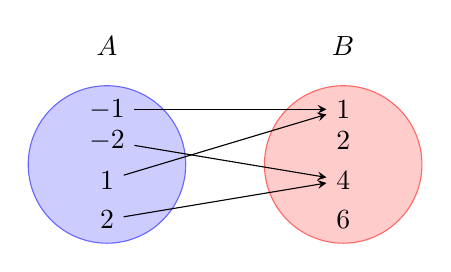
\begin{tikzpicture}
    % draw the sets
    \filldraw[fill=blue!20, draw=blue!60] (-1.5,0) circle (1cm);
    \filldraw[fill=red!20, draw=red!60] (1.5,0) circle (1cm);


    % the texts
    \node at (-1.5,1.5) {$A$};
    \node at (1.5,1.5) {$B$};

    % the points in the sets (here I just create nodes to use them later on to position
    % the circles and the arrows
    \node (x1) at (-1.5,0.7) {$-1$};
    \node (x2) at (-1.5,0.3) {$-2$};
    \node (x3) at (-1.5,-0.2) {$1$};
    \node (x4) at (-1.5,-0.7) {$2$};
    \node (y1) at (1.5,0.7) {$1$};
    \node (y2) at (1.5,0.3) {$2$};
    \node (y3) at (1.5,-0.2) {$4$};
    \node (y4) at (1.5,-0.7) {$6$};

    % draw the arrows
    \draw[->] (x1) -- (y1);
    \draw[->] (x2) -- (y3);
    \draw[->] (x3) -- (y1);
    \draw[->] (x4) -- (y3);

\end{tikzpicture}
\caption{Mapping diagram of $f$}
\end{figure}



Notice that we require the rule $f(a) = b$ to map each element $a$ to \emph{unique} elements $b$. This would of course imply that if a rule $f(a) = b$ assigns some $a$ more than one element in the co-domain, then we say that this rule $f(a) = b$ is $\textbf{not}$ a function.


\begin{defn}
Let $f$ be a function,

\begin{enumerate}
\item The \textbf{domain} $D$ of $f$ is the set of all $x$ such that $f(x)$ is well defined.
\item The \textbf{range} (or image) $R$ of $f$ is defined as $$R = \{f(x) \colon x\in D \}$$
\end{enumerate}

\end{defn}

\newpage


\begin{ex}
State the domain and range of $f$ in Figure 1.1
\end{ex}


\begin{soln}
Clearly the domain $D = A$, the range can be computed by determining all image points of $f$. We list them, $f(-1) = (-1)^2 = 1, f(-2) = (-2)^2 = 4, f(1) = 1^2 = 1, f(2) = 2^2 = 4$. Hence, $R = \{1,4\}$
\end{soln}

\vspace*{0.5cm}


\begin{ex}
State the domain for $f(x) = \sqrt{-3x - 9}$
\end{ex}


\begin{soln}
 We determine the set $D$ of all possible values of $x$ such that $f(x)$ is well defined. This occurs precisely when $-3x-9$ is a non-negative value, hence we require $-3x-9 \geq 0$ which would imply that $x \leq -3$. Hence the domain is any real number $x$ such that $x\leq -3$, or to put more concisely using set-builder notation $D = \{x\in R \colon x\leq -3 \}$ (Try to determine what the universe of discourse was here and the \textbf{statement} used).
\end{soln}


\vspace*{0.5cm}

\begin{ex}
State the domain and range for $f(x) = \frac{-3}{4}(x+3)^2 - 5$.
\end{ex}

\begin{soln}
Clearly $f$ is well defined for any $x\in \R$, hence $D = \{x\in \R\}$. Determining the range of $f$ can be tricky, I find the best way to determine the range is to quickly sketch the function, this is a parabola that has $y-$intercept = $-5$ and points \emph{downwards}, hence $R = \{y\in \R \colon y \leq -5 \}$.
\end{soln}


\end{document}
